\documentclass{article}
\usepackage{graphicx}
\usepackage{natbib}
\usepackage{doi}
\usepackage{float}
\usepackage{indentfirst}
\usepackage{setspace}



\title{Promega ML Paper}
\date{February 2026}

\author{
  Nicholas Ross\footnote{Data Science Institute, University of Chicago. \texttt{nickross@uchicago.edu}} \and
  Liya Ding\footnote{Data Science Institute and Center for Living Systems, University of Chicago. \texttt{liyading@uchicago.edu}} \and
  Tony Luo\footnote{Data Science Institute, University of Chicago. \texttt{tonyluo@uchicago.edu}} \and
  Harriet (Wenxu) Zu\footnote{Data Science Institute, University of Chicago. \texttt{harrietzu@uchicago.edu}} \and
  Lucy (Yihan) Li\footnote{Data Science Institute, University of Chicago. \texttt{yli24@uchicago.edu}} \and
  Ethan Waggoner\footnote{Data Science Institute, University of Chicago. \texttt{waggonere@uchicago.edu}}
}

\begin{document}
\maketitle

\begin{abstract}
Organoid quality assessment is often done through manual expert inspection, which is slow, expensive, difficult to scale, and subject to variability. We study whether organoid viability can be predicted automatically from data collected earlier in development. Our dataset contains 265 organoids observed across 12 time points from Day~3 to Day~30, with three complementary data sources: bright-field microscopy images, culture-medium metabolite measurements, and expert survey labels. The final binary outcome was derived from late-stage survey assessments. We propagated the label backward so that, for each culture day, we trained a separate classifier using only information available on that day to predict the organoid's final late-stage acceptability label. We compare three model families under shared train, validation, and test splits: an image-only model, a metabolite-only model, and a combined multimodal model. The image branch compares per-day and time-series formulations, the metabolite branch compares logistic regression with LightGBM, and the combined branch fuses image and metabolite features. Because the class distribution is imbalanced (72.5\% \textit{Acceptable}, 27.5\% \textit{Not Acceptable}), we use balanced accuracy as the primary evaluation metric. We find that predictive signal changes over the developmental timeline. The per-day image model performs strongly at early and middle time points and consistently outperforms the time-series image formulation. The metabolite model is weaker early but becomes the strongest late-stage predictor, reaching a balanced accuracy of 0.94 at Day~30. The combined model does not consistently outperform the best single modality at any given day. These results suggest that automated organoid screening can be tailored to developmental stage: image-based models provide broader earlier coverage, while metabolite-based models offer the strongest late-stage discrimination and a cheaper, more scalable alternative to repeated expert review.
\end{abstract}

\doublespacing

\section{Introduction}
Organoids are three-dimensional cell cultures that self-organize into structures resembling real tissues, making them a widely used platform for studying human development, disease, and drug response. Their scientific value depends critically on quality. However, quality assessment is typically performed through manual expert inspection: a process that is time-consuming, difficult to scale, and subject to inter-rater variability. Automated methods for reliable quality prediction are therefore an important practical need. This paper studies organoid quality prediction using a multimodal longitudinal dataset. The data set contains 265 organoids observed at 12 time points that span Days 3 through 30. Three sources of information are available for each organoid: brightfield microscopy images, metabolite concentration measurements from the culture medium, and expert survey labels indicating whether each organoid was ultimately judged \textit{Acceptable}. These modalities provide complementary views of the same biological system across development. 

For each culture day, we trained a separate classifier using only information available on that day to predict the organoid's final late-stage acceptability label. We develop and compare three families predictive models: an image-only model evaluating several computer vision backbones and comparing single-day versus time-series formulations, a metabolite-only model comparing logistic regression against LightGBM trained on concentrations and day-to-day differences, and a combined model fusing image and metabolite features through intermediate fusion. All models are evaluated using balanced accuracy as the primary metric given the imbalanced class distribution.

This paper makes three main contributions. First, we construct and analyze a longitudinal multimodal dataset that is larger and richer than most prior organoid studies, linking bright-field morphology, culture medium biochemistry, and expert quality labels across twelve time points for 265 organoids. Second, we provide a systematic comparison of image-only, metabolite-only, and combined models under a unified experimental framework that controls for class imbalance and ensures consistent data splits across modalities. Third, we show that predictive signals evolve over the developmental timeline: image-based models perform strongly across much of the growth period, metabolite-based models become substantially more informative at later stages, and combining the two modalities does not consistently improve over the best individual model at any given time point.

\section{Literature Review}

This paper lies at the intersection of organoid biology and machine learning for non-invasive quality prediction. The relevant literature suggests four linked points. First, organoids are increasingly important experimental systems, but their utility depends on reliable and reproducible quality assessment. Second, brightfield images contain meaningful morphological information that can be extracted through modern computer vision methods, including longitudinal image analysis over development. Third, metabolite measurements provide a complementary biochemical view of organoid state and can be modeled effectively with machine learning methods for structured data. Fourth, combining heterogeneous modalities is promising but methodologically challenging, especially under class imbalance. Together, these strands define the research landscape in which this paper is situated and clarify why longitudinal, multimodal organoid quality prediction is an important question.

\subsection{Organoids as Research Models and the Need for Quality Assessment}

Organoids have become an important model system because they reproduce key structural and functional features of living tissues while remaining experimentally accessible \textit{in vitro}. Broad reviews by Rossi et al., Zhao et al., and Tang et al.\ emphasize that organoids have expanded rapidly across developmental biology, disease modeling, drug testing, and translational research because they bridge the gap between traditional two-dimensional culture systems and more physiologically realistic tissue organization \cite{rossi2018,zhao2022,tang2022}. Organoids matter scientifically because they provide a flexible platform for studying human development and disease in a way that conventional cell culture often cannot.

At the same time, these reviews also make clear that organoid systems are marked by substantial heterogeneity. Variability can arise from cell sourcing, differentiation protocols, culture conditions, and developmental timing, all of which affect morphology, maturation, and functional fidelity \cite{rossi2018,zhao2022}. As organoid platforms scale, this variability becomes not merely a technical inconvenience but a central challenge for reproducibility and downstream use. Reliable quality assessment is therefore a necessary condition for using organoids as robust research and screening tools. In this sense, the problem addressed in this paper is directly tied to one of the field's persistent practical bottlenecks.

The literature also suggests that organoid quality should be understood as a developmental question rather than a purely static one. Pennington et al.\ show that metabolic processes such as glucose utilization and oxygen metabolism can actively shape developmental decisions, rather than simply reflecting passive byproducts of growth \cite{pennington2025}. Similarly, metabolomics-focused work in organoid systems emphasizes that organoids should be evaluated not only by morphology but also by whether they reproduce chemically meaningful states \cite{murphy2022}. Together, these studies motivate the central premise of this paper: whether an organoid will ultimately be judged \textit{Acceptable} may be reflected in measurements collected earlier in development, including both morphology and biochemical state.

\subsection{Image-Based Analysis of Organoid Development}

A growing body of work shows that organoid images contain biologically informative signal that can be analyzed computationally. Park et al.\ provide direct evidence that deep learning can support automated organoid image analysis from microscopy data, including image segmentation and morphology-aware processing \cite{park2023}. This supports the use of brightfield images not merely as visual documentation, but as a data source from which biologically meaningful features can be extracted. The image branch of this paper rests on this established premise: organoid morphology visible in microscopy images contains information that is potentially predictive of downstream biological outcomes.

Recent work also shows that organoid imaging is particularly informative when studied longitudinally rather than at a single isolated time point. Sockell et al.\ demonstrate that high-throughput imaging can be used to track organoids over time and recover phenotypic trajectories linked to later molecular and functional properties \cite{sockell2023}. This longitudinal perspective is important for the present study because organoid quality is not expected to become fully visible at the earliest stages of growth. Instead, it may emerge gradually as morphology matures. This motivates the comparison in this paper between single-day and time-series image models regarding whether images from the past development trajectory contain predictive information beyond any one snapshot.

The present image-prediction task also fits into a broader machine-learning framework for longitudinal biomedical data. Cascarano et al.\ describe settings in which repeated measurements are used to predict a later or static outcome, a structure that closely matches the label construction used in this paper \cite{cascarano2023}. The final expert quality label is assigned from late-stage assessment and propagated backward, while the models are asked to predict that eventual label using information available at earlier time points.

Finally, the image literature has evolved alongside advances in general-purpose visual backbones. Convolutional architectures remain central to biomedical image analysis, but transformer-based encoders have become increasingly important in computer vision. Dosovitskiy et al.\ introduced the Vision Transformer (ViT), showing that pure transformer architectures applied to image patches can perform competitively on image-classification tasks \cite{dosovitskiy2021}. Such developments help explain why both convolutional and transformer-based backbones are reasonable candidates in the image-model comparison.

\subsection{Metabolite Measurements as Predictors of Organoid State}

Where images capture morphology, metabolite measurements provide a complementary biochemical view of organoid development. Murphy and Sweedler argue that organoid evaluation should account not only for structural resemblance to native tissue but also for the chemical environment and metabolic state of the system \cite{murphy2022}. The metabolite branch of this paper is inspired by this finding that culture-medium chemistry can provide meaningful information about whether an organoid is developing appropriately.

This biological argument is strengthened by developmental studies linking metabolism to cell-state transitions and developmental outcomes. Pennington et al.\ suggest that metabolic dynamics are intertwined with developmental processes rather than merely secondary to them \cite{pennington2025}. From the perspective of this paper, this means that longitudinal metabolite measurements may carry predictive signal about eventual organoid acceptability, especially if biochemical differences emerge before visual differences become obvious.

The machine-learning literature also supports the use of predictive models for structured metabolomic data. She et al.\ show that metabolomics combined with machine learning can identify diagnostic and prognostic biomarkers in a biomedical setting \cite{she2023}. Guldogan et al.\ further demonstrate that LightGBM, paired with SHAP-based interpretation, can perform effectively on serum metabolomics while also highlighting biologically informative features \cite{guldogan2025}. These studies support two methodological choices that are relevant here: first, tabular metabolite measurements are well suited to nonlinear machine-learning models; second, interpretability can be valuable when the goal is not only classification but also identifying which biochemical signals matter most.

Wang et al.\ provide additional support for the practical strength of LightGBM in biomedical prediction, although in a different domain involving radiomics and clinical features rather than metabolomics alone \cite{wang2024}. Taken together, these studies do not imply that one particular algorithm is universally optimal, but they do justify the general modeling strategy adopted in this paper: structured metabolite data can be treated as a predictive modality in their own right, and gradient-boosted tree methods are a reasonable and well-supported choice for that setting.

\subsection{Multimodal Learning, Class Imbalance, and Thresholding}

If morphology and metabolite profiles capture different aspects of organoid development, then combining them is a natural next step. The multimodal-learning literature suggests that heterogeneous data sources often contain complementary information, but that effective fusion depends on how those sources are aligned and represented. Gao et al.\ survey deep learning for multimodal data fusion and emphasize that modalities may differ in dimensionality, structure, and noise characteristics, making fusion a methodological problem rather than a trivial concatenation step \cite{gao2020}. This observation is directly relevant to the present study, where image-derived features and metabolite features differ sharply in representation and scale.

Related biomedical studies reinforce the idea that multimodal models can improve prediction when modalities carry partially distinct signal. De Palma et al., for example, show that combining heterogeneous biomedical features can improve prognostic modeling in a setting where no single modality is complete on its own \cite{depalma2026}. For this paper, the multimodal hypothesis is analogous. An organoid that appears ambiguous in morphology may nonetheless exhibit informative metabolite patterns, and vice versa.

A second major methodological issue is class imbalance. In this dataset, the \textit{Acceptable} class is substantially larger than the \textit{Not Acceptable} class, so overall accuracy alone can be misleading. Abdelhamid and Desai show that imbalance-aware methods such as class weighting, oversampling, and threshold calibration can materially improve minority-class performance in binary classification \cite{abdelhamid2024}. This literature supports the methodological emphasis in this paper on balanced accuracy, class weighting, and other procedures that prevent the majority class from dominating evaluation.

Threshold choice is especially important in imbalanced settings. Esposito et al.\ show that the default decision threshold of 0.5 is often suboptimal under class imbalance and that threshold adjustment can improve minority-class detection without retraining the model \cite{esposito2021}. This is directly relevant to the image branch of the present study, where threshold analysis is treated as part of the substantive evaluation.

\subsection{Summary}

The literature suggests a clear research trajectory. Organoids are scientifically valuable but highly variable, making quality assessment a central practical problem. Prior work shows that brightfield images can support organoid analysis and longitudinal phenotyping, while metabolite measurements provide a complementary biochemical view of developmental state. At the same time, multimodal fusion, class imbalance, and threshold selection introduce methodological challenges that cannot be ignored if the goal is reliable screening.

This paper fits into that landscape by asking a more specific question than most prior studies have addressed directly: whether longitudinal morphology and longitudinal biochemical state can be used, separately and jointly, to predict eventual organoid acceptability. To answer that question, this paper compares image-only, metabolite-only, and combined models using repeated measurements across development and evaluates them under imbalance-aware metrics and threshold analysis. In doing so, it places organoid quality prediction within a multimodal and longitudinal machine-learning framework while addressing a practical problem of clear relevance to organoid-based research.


\section{Data}

This paper studies organoid quality prediction using a multimodal dataset that combines longitudinal bright-field imaging, metabolite measurements from culture medium, and expert survey-based quality assessments. At the biological level, organoids were observed over 12 time points: Days 3, 6, 8, 10, 13, 15, 17, 20.5, 24, 26, 28, and 30. During data integration, Days 20 and 21 were mapped to Day 20.5 to improve consistency across experiments. There was also no Day 26 in the metabolite data. These measurements were assembled into a unified normalized-record system that merged image data, metabolite data, survey information, segmentation metadata, and day-specific identifiers into a single standardized structure. In the final unified dataset, the main \texttt{all\_data.json} file contained 5,168 total image records, while the day-indexed image-classifier view contained 2,931 labeled image records across 11 modeled days.

\begin{figure}[H]
    \centering
    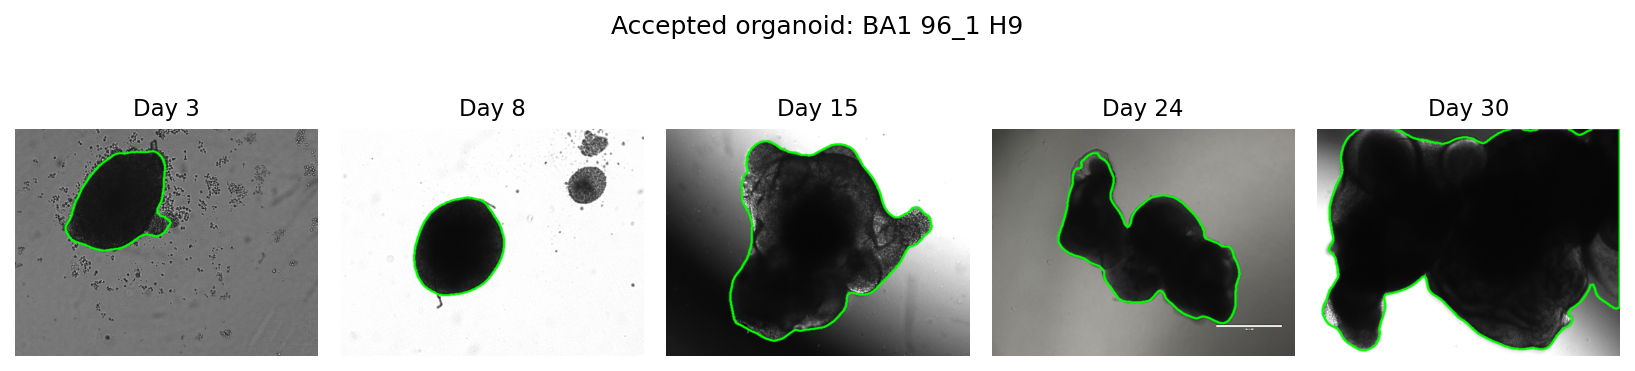
\includegraphics[width=1.0\linewidth]{Images/1_organoid_overlay_strip.png}
    \caption{Example of an acceptable organoid tracked across development from Day 3 to Day 30. The green overlay marks the segmented boundary used in the image pipeline.}
\end{figure}

This multimodal organization is central to the logic of the study. Image data capture changes in organoid morphology over time while metabolite data provide a complementary biochemical view of organoid development. The late-stage expert surveys serve as the supervisory signal that ties both modalities to the same practical target: whether an organoid would ultimately be judged \textit{Acceptable} by human evaluators.

\subsection{Image Quality Issues}

A central challenge in the raw microscopy image data was recurring quality issues that are not themselves biological signals, but could nevertheless affect downstream classification if left unaddressed. The most important issues are stitching, splitting, the Day 30 red scale bar, and progressively stronger shadowing in later-stage images.

The first issue is \textit{stitching}. Some organoids are large enough that the imaging system captures them through multiple adjacent fields, which are then stitched into a single image. This stitching process can introduce visible irregularities and, in some cases, produces the black-box artifact seen in the raw images. The second issue is \textit{splitting}. As an organoid grows, it may split into two daughter organoids, so later image records can represent branches of the same original developmental history rather than fully independent samples. This creates an additional challenge for longitudinal analysis, because the dataset must distinguish between true time-series continuity and trajectories that diverge after a split event. The pipeline therefore tracks split organoids explicitly during image mapping and genealogy-based series construction so that downstream analyses can handle these related records appropriately. A third issue is the \textit{red scale bar}, which appears on Day 30 images. Although visually small, it introduces a fixed graphical element that is unrelated to organoid morphology and could be spuriously learned by a classifier. Finally, later-stage images often exhibit substantially stronger \textit{shadowing} than earlier-stage images. This creates an important tension in the image branch of the project: organoid quality becomes more visible as organoids mature, but the later images are also less visually uniform and more affected by acquisition-related artifacts.

\begin{figure}[H]
    \centering
    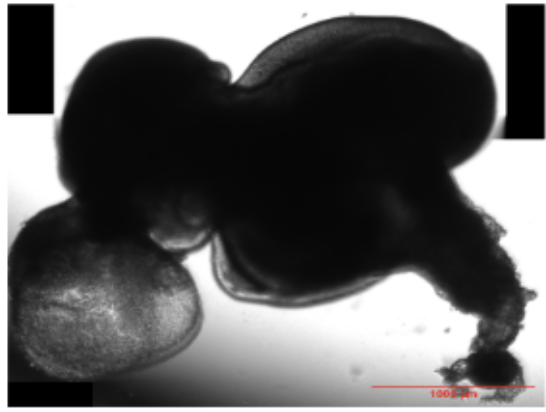
\includegraphics[width=0.3\textwidth]{Images/3_5_stitched_red_bar.png}
    \caption{Example of a stitched organoid image. Stitching can introduce visual irregularities and black-box artifacts, while Day 30 images may also contain a red scale bar unrelated to organoid morphology.}
\end{figure}

\begin{figure}[H]
    \centering
    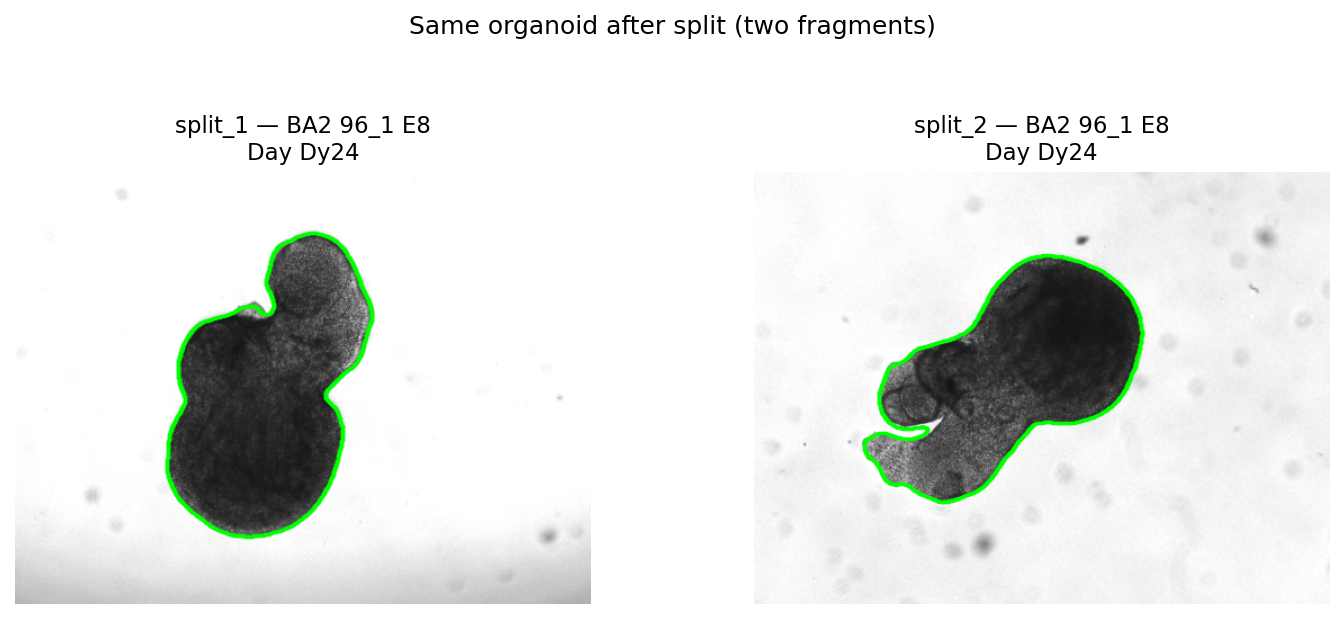
\includegraphics[width=0.7\textwidth]{Images/4_same_organoid_split.png}
    \caption{Example of a split event in which one organoid gives rise to two daughter fragments at a later time point. Such cases complicate longitudinal analysis because later images no longer correspond to a single uninterrupted trajectory.}
\end{figure}

\begin{figure}[H]
    \centering
    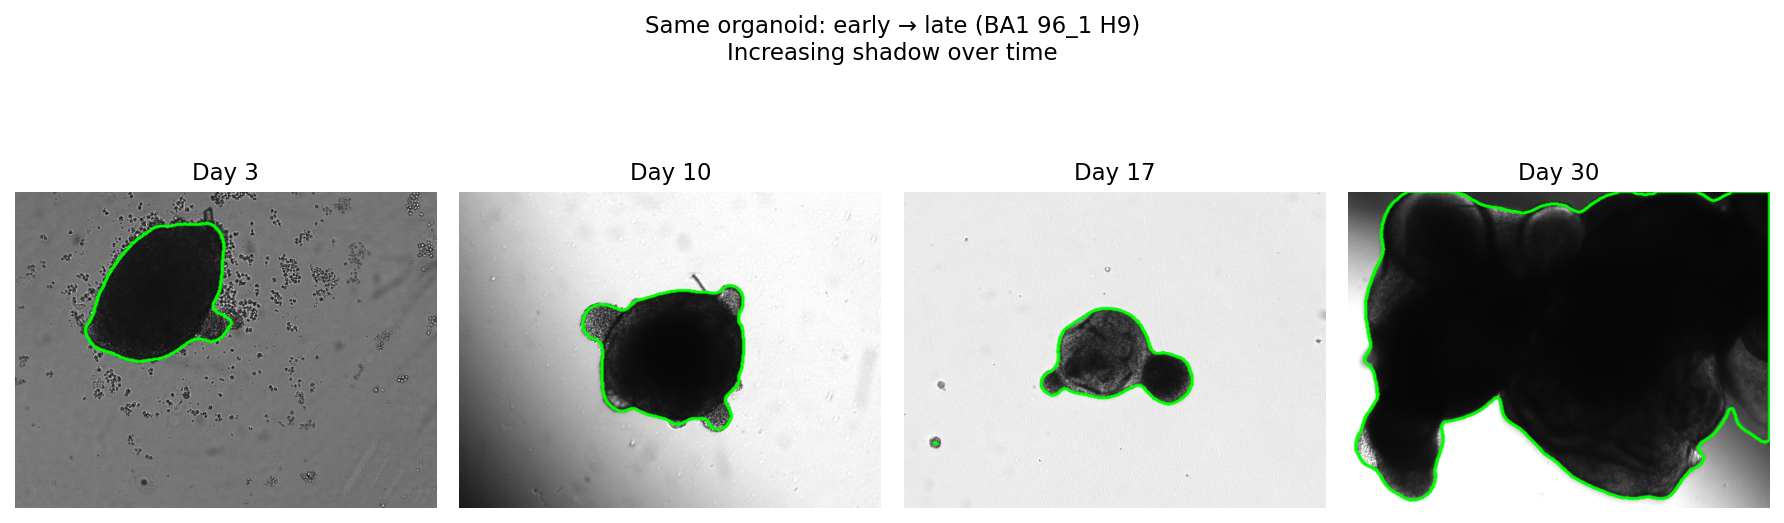
\includegraphics[width=\textwidth]{Images/6_shadow_contrast_4timepoints.png}
    \caption{Example of the same organoid across development, illustrating progressively stronger shadowing at later time points. This creates a tension in the image branch: later-stage morphology is more informative, but image quality is less uniform.}
\end{figure}

These image-quality issues motivated the design of the preprocessing pipeline, including the overlay representations, separate segmentation models for early and late stages, resizing and aspect-ratio standardization, and later background-normalization steps. These steps were introduced to suppress non-biological variation and make organoid boundaries and overall morphology more salient to the classifier.

\subsection{Metabolite Data}

The metabolite branch used repeated measurements from culture medium, including GlucoseGlo, GlutamateGlo, LactateGlo, MalateGlo,\footnote{MalateGlo was available from Day 13 onward.} and PyruvateGlo. Table~\ref{tab:metabolites} summarizes the five metabolites used as predictive features.

\begin{table}[H]
\centering
\renewcommand{\arraystretch}{1.4}
\begin{tabular}{|l|r|r|r|r|}
\hline
\textbf{Metabolite} & \textbf{Mean} & \textbf{Min} & \textbf{Max} & \textbf{Std. Dev.} \\
\hline
Glucose concentration ($\mu$M)   & 11.612 & $-$0.083 & 19.920 & 2.597 \\
\hline
Glutamate concentration ($\mu$M) &  1.289 &    0.024 & 22.902 & 1.008 \\
\hline
Lactate concentration ($\mu$M)   & 10.791 &    0.059 & 46.680 & 6.647 \\
\hline
Pyruvate concentration ($\mu$M)  &  2.820 & $-$0.462 &  6.738 & 0.865 \\
\hline
Malate concentration ($\mu$M)    &  0.120 & $-$0.167 & 26.818 & 0.772 \\
\hline
\end{tabular}
\caption{Summary statistics of metabolite concentrations across organoid IDs and timepoints.}
\label{tab:metabolites}
\end{table}

Figure~\ref{fig:boxplots} shows the distribution of metabolite concentrations across organoid samples. Glucose and lactate show the highest concentration levels and the widest variability, indicating substantial differences across organoid samples. In contrast, glutamate and pyruvate appear at lower concentrations with comparatively tighter distributions. Malate concentrations are generally very low and display minimal variation; notably, malate measurements only appear after Day 10, reflecting its later emergence in the experimental timeline. Overall, these distributions highlight differences in both magnitude and variability across metabolites, which may influence their usefulness as predictive features.

\begin{figure}[H]
\centering
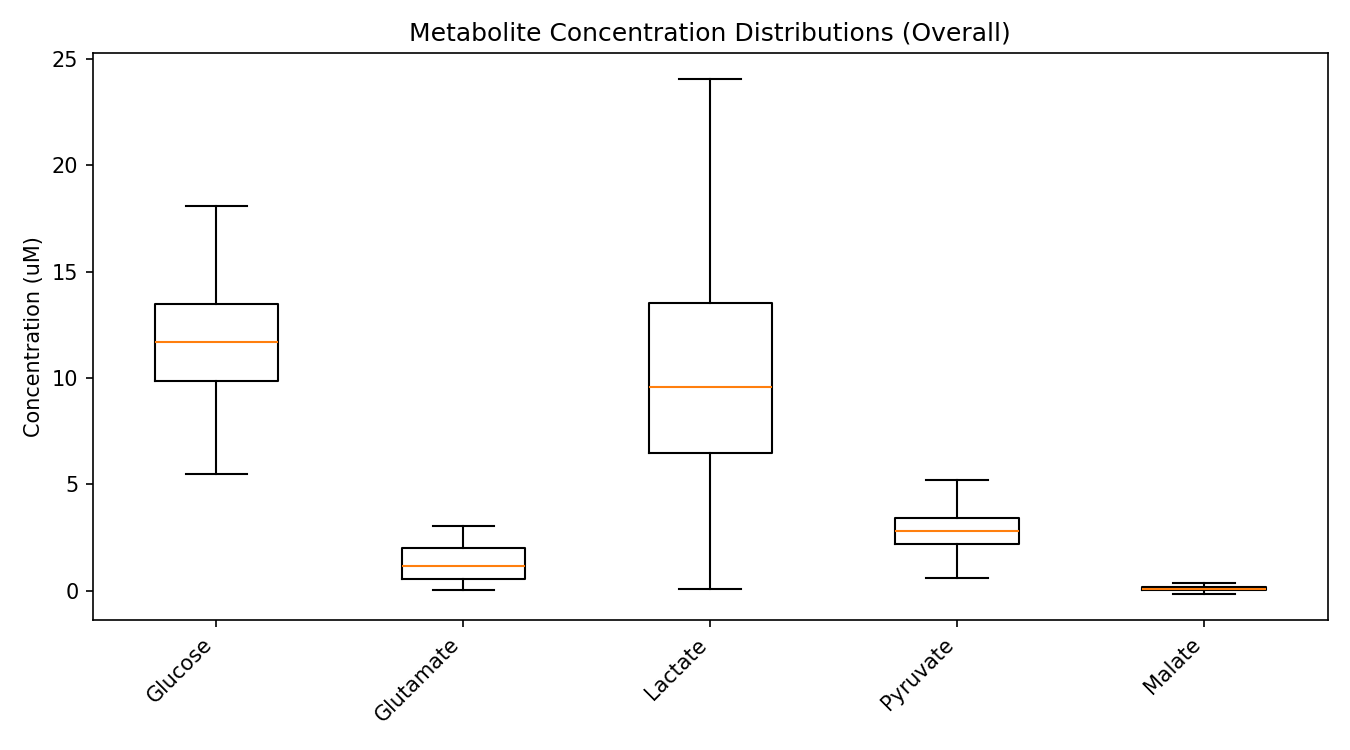
\includegraphics[width=\textwidth]{Images/metabolite_concentration_boxplot.png}
\caption{Boxplots showing the distribution of metabolite concentrations across organoid samples.}
\label{fig:boxplots}
\end{figure}

On top of concentrations, for each organoid, the day-to-day difference in metabolite concentration was computed as the numerical change in each metabolite's micromolar concentration between consecutive observation days. For a given metabolite $m$ and organoid $i$, the difference feature at day $t$ was defined as $$\Delta c_{i,m}(t) = c_{i,m}(t) - c_{i,m}(t_{\mathrm{prev}}),$$ where $c_{i,m}(t)$ denotes the measured concentration of metabolite $m$ for organoid $i$ at day $t$, and $t_{\mathrm{prev}}$ is the immediately preceding observation day for that organoid. 

\subsection{Label generation}

The prediction target was derived from expert survey assessments of organoid quality. Each organoid was evaluated by five human raters using \textit{Acceptable} versus \textit{Not Acceptable} judgments. To ensure that the final labels reflected strong agreement rather than marginal preference, the labeling system required at least four matching votes, corresponding to an 80\% consensus threshold. Labels assigned from the late-stage Day 28/30 surveys were then propagated backward to all earlier time points for the same organoid.

\begin{figure}[H]
    \centering
    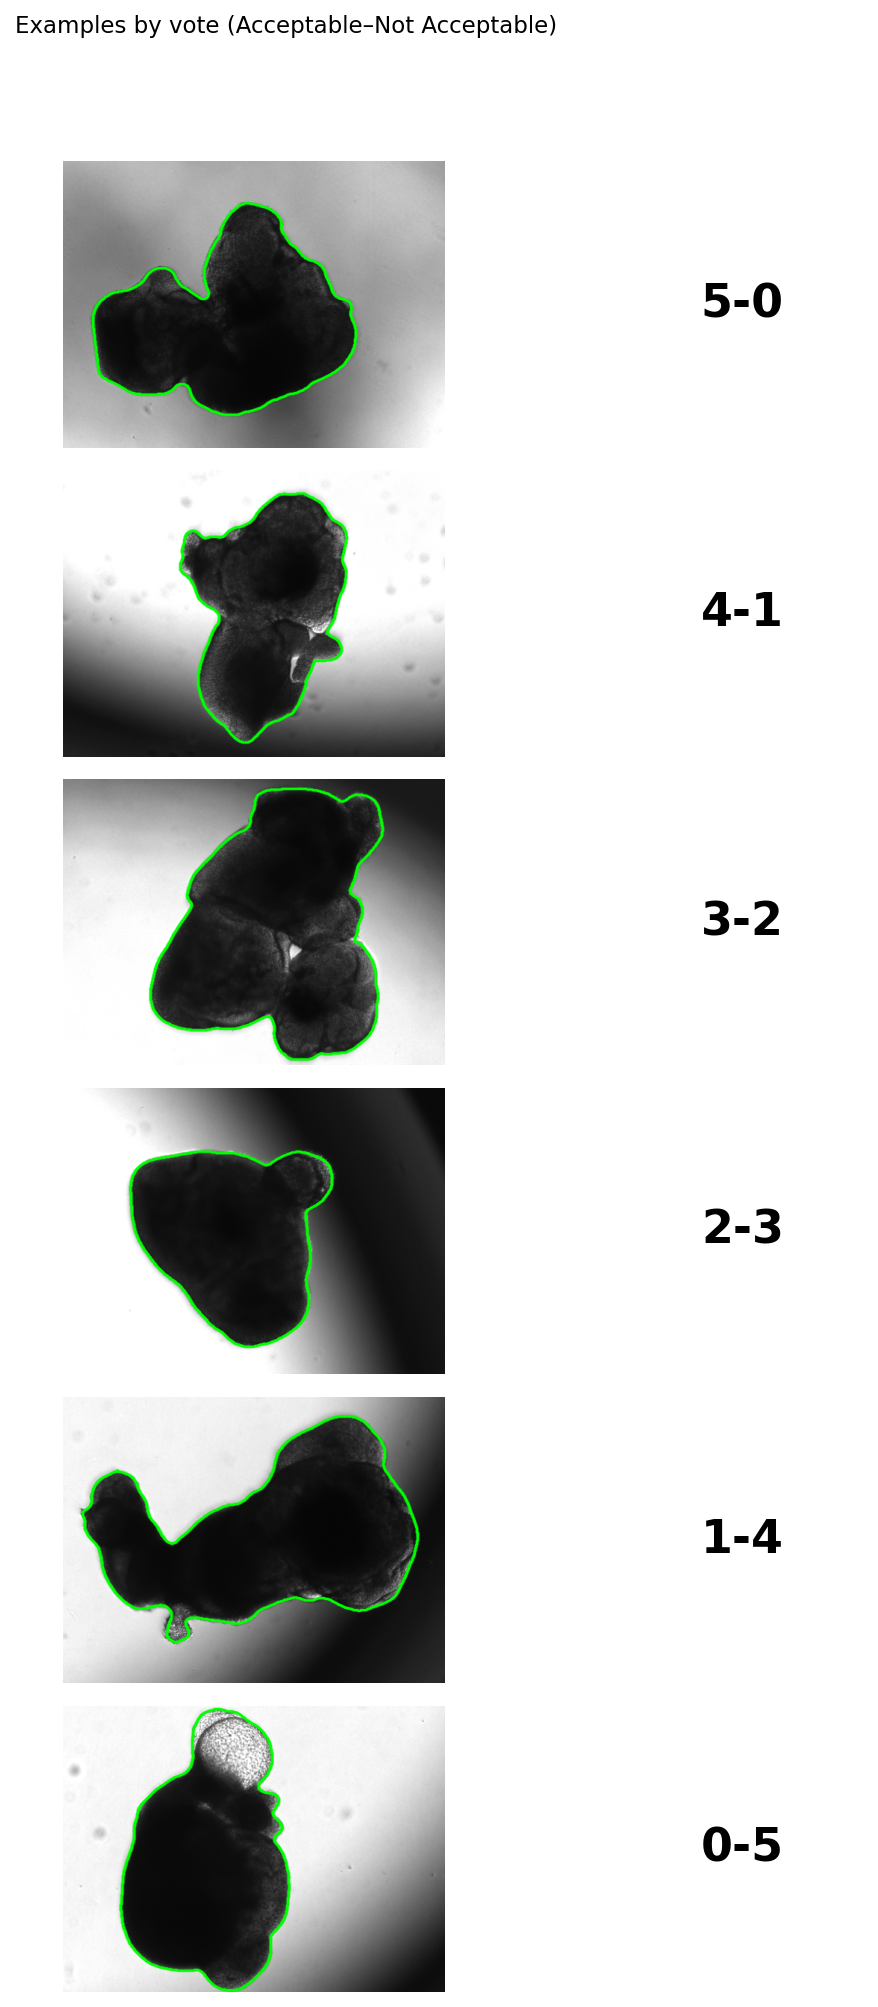
\includegraphics[height=0.7\textheight]{Images/2_organoid_vote_table.png}
    \caption{Representative examples of organoids by expert vote pattern, from unanimous \textit{Acceptable} (5--0) to unanimous \textit{Not Acceptable} (0--5). This illustrates the range of visual ambiguity underlying the final binary labels.}
\end{figure}

The labeled image dataset contained 265 unique organoids and 2,931 labeled image records across the 11 modeled days. After propagation, the labels were fully consistent across time points, and 13 organoids with conflicting labels across days or splits were removed. The resulting class distribution was imbalanced, with 72.5\% of organoids labeled \textit{Acceptable} and 27.5\% labeled \textit{Not Acceptable}. This imbalance is important because a model could achieve seemingly strong overall accuracy by favoring the majority class while still performing poorly on the minority class, which is often of particular practical interest in screening.

For this reason, this paper uses balanced accuracy as the primary evaluation metric. Balanced accuracy is defined as the average of sensitivity and specificity,
\[
\mathrm{Balanced\ Accuracy}=\frac{\mathrm{Sensitivity}+\mathrm{Specificity}}{2},
\]
so that performance on the \textit{Acceptable} and \textit{Not Acceptable} classes receives equal weight despite the uneven class distribution. This makes balanced accuracy a more informative summary metric than ordinary accuracy for the present classification task.

\subsection{Train/validation/test splitting}

Model development used explicit train/validation/test splits constructed from the resized image mapping JSON. The default split proportions were 80\% training, 10\% validation, and 10\% test. During split generation, 36 problematic bad entries were removed, leaving 5,132 resized image records available for assignment.

The same split structure was then reused across the image and metabolite model training. This is methodologically important: because all backbone comparisons and later threshold studies used the same base split files, differences in model performance can be interpreted as differences in modeling strategy rather than artifacts of changing data partitions. This shared split design therefore supports clean comparisons across architectures, input modes, and temporal formulations. 

\section{Models}
\subsection{Model \#1: Images}

\subsubsection{Description of Three Models}

The initial image-model comparison considered three legacy backbones: ViT, ResNet50, and EfficientNet-B0. All three models solved the same binary classification task, with \textit{Acceptable} encoded as 1 and \textit{Not Acceptable} encoded as 0, using per-day image inputs. Although the architectures differed, the comparison was designed to be as fair as possible by holding the rest of the training pipeline fixed.

Across all three models, the shared setup was as follows. Inputs were drawn from fixed train/validation/test split JSON files, and for each modeled day the pipeline extracted the corresponding image paths and labels. Images were resized to $512 \times 384$ pixels, implemented in code as \texttt{Resize(384, 512)}. The default batch size was 16. Training augmentation included random horizontal flips and mild color jitter. All three models used focal loss with $\gamma = 2.0$ and $\alpha = 0.25$, together with balanced class weights to mitigate label imbalance. Optimization followed a two-phase schedule: first the backbone was frozen and only the classifier head was trained using Adam with learning rate $10^{-3}$, then deeper backbone layers were partially unfrozen and fine-tuned using Adam with learning rate $10^{-4}$. Training also used a \texttt{ReduceLROnPlateau} scheduler and early stopping. For each day, the best checkpoint was selected by validation accuracy.

The three models differ primarily in how they encode visual information. ViT used a DINOv2-base transformer backbone, in which the image is represented through patch embeddings and a CLS token that serves as the global feature vector. A small classifier head maps that feature vector to the probability of the \textit{Acceptable} class. ResNet50 used a standard convolutional backbone with hierarchical feature extraction followed by global average pooling and a multilayer perceptron classifier head. EfficientNet-B0 likewise used a convolutional backbone, but one designed to balance depth, width, and resolution more efficiently than a conventional ResNet. In all three cases, the backbone served as a learned feature extractor and the final head produced a single binary prediction.

\subsubsection{EfficientNet as the Best Model}

Among the three legacy backbones, EfficientNet-B0 emerged as the strongest overall model. The summary table below shows that EfficientNet achieved the highest average true negative rate across all days (29.1\%), the highest early-day true negative rate over Days 3--10 (12.5\%), the highest balanced accuracy (59.0\%), the fewest days with TNR equal to zero (2/11), and the highest F1 score for the \textit{Not Acceptable} class (29.2\%). By contrast, ViT and ResNet were both weaker on these criteria, especially in identifying the minority \textit{Not Acceptable} class.

This paper therefore treats EfficientNet-B0 as the primary image backbone. That choice is especially well motivated in the present setting, where the practical screening problem depends not only on identifying clearly \textit{Acceptable} organoids, but also on avoiding missed detections in the more difficult \textit{Not Acceptable} class. Since the class distribution is imbalanced, the stronger TNR and balanced-accuracy profile of EfficientNet is more informative than ordinary accuracy alone.

\begin{table}[htbp]
\centering
\small
\setlength{\tabcolsep}{5pt}
\begin{tabular}{lccccc}
\hline
\textbf{Model} & \textbf{Avg. TNR} & \textbf{Early TNR} & \textbf{Bal. Acc.} & \textbf{Days} & \textbf{F1} \\
               & \textbf{(All)}    & \textbf{(Dy3--10)} &                   & \textbf{TNR = 0} & \textbf{(N.A.)} \\
\hline
ViT          & 23.7\% & 4.2\%  & 58.0\% & 4/11 & 24.7\% \\
ResNet       & 20.5\% & 0.0\%  & 57.2\% & 5/11 & 21.4\% \\
EfficientNet & 29.1\% & 12.5\% & 59.0\% & 2/11 & 29.2\% \\
\hline
\end{tabular}
\caption{Cross-model comparison of the three legacy image backbones. Metrics emphasize minority-class performance on the \textit{Not Acceptable} class.}
\label{tab:legacy_model_comparison}
\end{table}

After this baseline comparison, the image pipeline was further refined through an improved EfficientNet training procedure explicitly optimized for better \textit{Not Acceptable} detection. This improved version retained EfficientNet-B0 as the backbone, but changed the model-selection rule from validation accuracy to validation balanced accuracy, increased the weight on the minority \textit{Not Acceptable} class by a factor of 2.5, lowered the focal-loss $\alpha$ parameter from 0.25 to 0.15, monitored TNR and TPR directly during training, and introduced stronger augmentation including vertical flips, rotation, affine translation, perspective transforms, and stronger color jitter. These changes were motivated by quality-control risk: in this application, failing to identify a poor-quality organoid can be more consequential than an ordinary classification error.

\begin{figure}[htbp]
  \centering
  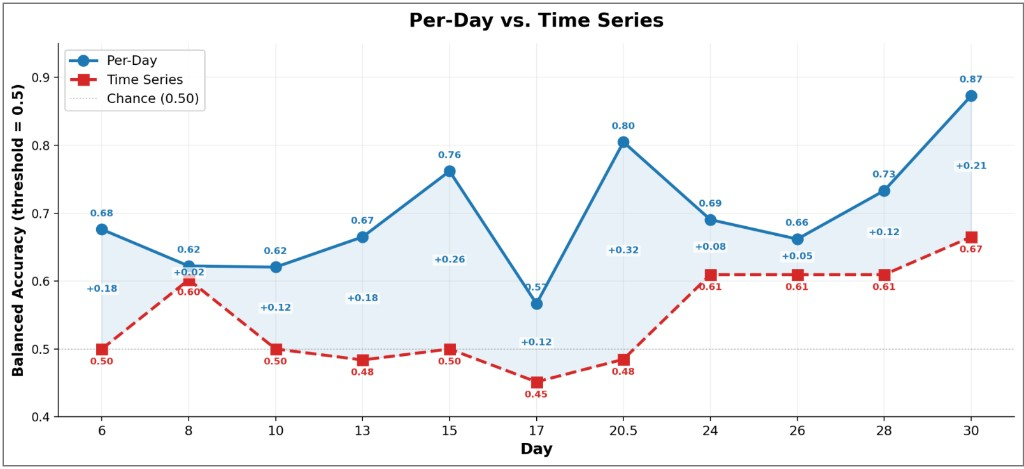
\includegraphics[width=0.85\textwidth]{Images/perday_vs_timeseries.png}
  \caption{Per-day classifier versus time-series classifier: balanced accuracy across culture days at a fixed decision threshold of 0.5. The per-day model (single image per day) consistently outperformed the time-series model (accumulated image sequence from Day~6).}
  \label{fig:perday_vs_timeseries}
\end{figure}

\subsubsection{Per Day and Times Series}

Once EfficientNet had been established as the preferred backbone, the next question was whether organoid quality is better predicted from a single image at a given day or from the accumulated developmental trajectory up to that day. To answer this, the project compared two EfficientNet-based formulations under a common overlay-image setup.

This comparison also involved a change in training strategy. The earlier improved TNR-focused EfficientNet was selected and tuned to emphasize minority-class detection. In the later per-day and time-series comparison, model selection was instead based on validation balanced accuracy, and training used standard binary cross-entropy with class weights. This shift was intended to provide a cleaner comparison between single-day and temporal modeling strategies.

In the \textit{per-day} setting, one EfficientNet classifier was trained for each day using only that day's image. This design tests whether morphology at a given moment is already sufficient to predict the final propagated label.

In the \textit{time-series} setting, one model was trained for each cutoff day using all images from Day 6 up to that day as an accumulated sequence. This design tests whether developmental history contains predictive information beyond what is visible in a single snapshot. Because organoid morphology becomes more informative as maturation proceeds, the comparison between per-day and time-series models directly tests whether the trajectory itself adds value or whether the latest image already captures most of the relevant signal.

\subsubsection{Thresholding}

Threshold choice plays an important role in interpreting image-model performance, especially because the dataset is imbalanced and the practical objective includes reliable detection of the \textit{Not Acceptable} class. The image comparison therefore evaluated thresholds from 0.5 to 0.9 and also considered optional validation-based threshold tuning.

In the legacy image-classification pipeline, binary predictions were obtained by applying a sigmoid function to the model output and thresholding at 0.5. The improved EfficientNet pipeline likewise used a default cutoff of 0.5, but its training procedure was explicitly oriented toward better minority-class detection through balanced-accuracy model selection, minority-class reweighting, focal loss, and direct monitoring of TNR and TPR. This makes threshold analysis especially important: once a model has been trained, sensitivity and specificity can often be rebalanced further by adjusting the decision threshold, even without retraining the underlying network.

For this reason, the threshold study in this paper should be understood as complementary to model training. The improved EfficientNet pipeline already shifts the learned classifier toward stronger \textit{Not Acceptable} detection, while the threshold sweep provides an additional way to study how the final operating point changes the tradeoff between true positive and true negative performance.

\subsection{Model \#2: Metabolites}
\subsubsection{Description of Two Models}

We evaluated two metabolite-only classifiers for organoid quality prediction at each observation day: a logistic regression baseline and a LightGBM model. In both cases, the prediction task was binary classification of organoids into \textit{Acceptable} and \textit{Not Acceptable} classes using metabolite measurements from the culture medium.

The logistic regression model served as a deliberately simple baseline. It gave us a linear reference point that was easy to interpret and useful for asking whether the metabolite signal was already separable with a low-capacity classifier. However, this baseline imposed a strong structural assumption: each metabolite feature contributed additively and linearly on the log-odds scale. That assumption was restrictive for this setting, where biological state may be reflected not only in absolute metabolite levels but also in nonlinear thresholds and interactions across metabolites.

The second model was LightGBM, a gradient-boosted tree method for tabular data. We selected this family because it can represent nonlinear decision boundaries, handle feature interactions without explicit manual construction, and remain well matched to a moderate-sized structured feature space. This made it a more natural candidate to explore whether they were separable in a biologically plausible way that was not necessarily linear.

For both models, we adopted a per-day training design. That is, for each culture day, we trained and evaluated a separate classifier using only observations available for that day. We chose this design for two reasons. First, it aligned the metabolite pipeline with the image pipeline, making day-by-day comparisons straightforward. Second, it avoided forcing a single temporal model to assume that metabolite information should accumulate monotonically over time. In this application, that assumption was not well justified: the biological meaning of day-to-day chemical changes is less naturally cumulative than the progressive visual differentiation seen in late-stage morphology.

\subsubsection{LightGBM with concentration differences}

Metabolite concentrations provide a snapshot of the chemical state of each organoid at a given day, but the day-over-day differences add information about how that state is changing. Our final metabolite model  used LightGBM trained on absolute concentrations as well as differences, computed for each metabolite as the numerical change from the previous available day. These features are not intended to represent biological growth rates; rather, they capture short-interval chemical movement in the culture medium. That information is useful because two organoids can have similar absolute concentrations at a given day while still following different trajectories of glucose consumption or metabolite accumulation. By encoding whether a metabolite is rising, falling, or remaining relatively stable from one observation to the next, the difference features give the model access to recent directional change that raw concentration values alone may miss. In practice, this helps distinguish organoids that appear similar in static metabolite space but differ in the pace or direction of their metabolic shift, which is exactly the kind of nonlinear pattern a tree-based model such as LightGBM can exploit.

For each day-specific model, we tuned LightGBM with a stratified search over a compact CPU-based hyperparameter grid. We intentionally used a small search rather than an expansive one. Given the size of the dataset and the relatively small number of \textit{Not Acceptable} examples at each day, a very large hyperparameter search would have increased variance and engineering complexity more than it would have improved the scientific clarity of the model. Our goal was not to exhaust the search space, but to identify a stable model family whose performance gains could be attributed to better inductive fit rather than to aggressive optimization.

The final training configuration used class weighting to address label imbalance: the \textit{Not Acceptable} class receiving additional emphasis during fitting. This choice was important because overall accuracy could otherwise be dominated by the larger \textit{Acceptable} class. We paired this with a model-selection objective focused on the F1 score for the \textit{Not Acceptable} class, and we used the same class-specific objective during threshold tuning. This design reflected two priorities of the task: first, identifying poor-quality organoids was more important than marginal gains on the majority class, and second, the dataset was unevenly distributed, with substantially fewer \textit{Not Acceptable} examples than \textit{Acceptable} ones. That imbalance made minority-class failures easy to hide behind strong overall accuracy, so we explicitly prioritized training and thresholding choices that forced the model to pay attention to the rarer but more consequential errors. At the same time, by using F1 rather than recall alone during model selection, we avoided pushing the classifier toward an overly permissive decision rule that would identify too many \textit{Acceptable} organoids as \textit{Not Acceptable}.

\subsubsection{Model selection rationale}

\begin{table}[H]
\centering
\renewcommand{\arraystretch}{1.4}
\begin{tabular}{|l|r|r|r|r|r|}
\hline
\textbf{Model} & \textbf{Avg. Accuracy} & \textbf{Avg. Bal.\ Acc.} & \textbf{Avg. Recall (N.A.)} & \textbf{Days Recall\textsubscript{NA}$= 0$} & \textbf{Best Bal.\ Acc.} \\
\hline
Logistic Regression & 83.3\% & 52.9\% & 15.9\% & 7/11 & 74.5\% \\
\hline
LightGBM            & 86.0\% & 60.9\% & 39.3\% & 1/11 & 94.4\% \\
\hline
\end{tabular}
\caption{Comparison of the two metabolite classifiers aggregated across all 11 modeled days.}
\label{tab:metabolite_model_comparison}
\end{table}

Table~\ref{tab:metabolite_model_comparison} summarizes the aggregate comparison between the two metabolite classifiers. Across all 11 modeled days, LightGBM achieved a higher average balanced accuracy (60.9\% versus 52.9\%), a substantially higher average recall for the \textit{Not Acceptable} class (39.3\% versus 15.9\%), and produced zero minority-class recall on only 1 of 11 days compared with 7 of 11 for logistic regression. LightGBM also reached a best-day balanced accuracy of 94.4\% at Day~30, compared with 74.5\% for logistic regression at Day~24. Although the two models achieved similar overall accuracy (a difference of roughly three percentage points), the gap in balanced accuracy and minority-class recall shows that LightGBM's advantage lay specifically in detecting \textit{Not Acceptable} organoids rather than in classifying the already well-separated majority class.

\subsection{Model \#3: Combined}
\subsubsection{Combined Model Design Strategies}

We designed a multimodal classifier that fused image-derived and metabolite-derived features to predict organoid quality (\textit{Acceptable} vs.\ \textit{Not Acceptable}). The combined model was motivated by the hypothesis that morphology (captured by images) and chemical state (captured by metabolite concentrations) provided complementary signals; combining them could improve discrimination. 

Two main design choices were made. First, we used the same train/ validation/ test splits and day definitions as the image-only and metabolite-only pipelines, so that all comparisons were aligned and no information leaked across splits. Second, we adopted a per-day training setup: for each day (e.g., Day 06, Day 10, \ldots, Day 30), we trained a separate combined classifier. This mirrored the per-day image and metabolite models and allowed performance to be reported and compared at each time point.

\subsubsection{Feature Extraction and LightGBM}


The combined pipeline had four stages: metabolite feature extraction, image feature extraction, dimensionality reduction, and classification. In the section below each was discussed in order.

For each organoid on each day, 10 metabolite-derived features were taken just as in the metabolite model.

The pretrained EfficientNet (no fine-tuning) was used as a fixed feature extractor for our model, and all the setup remained the same as the per-day model. The time-series model was not used here; the combined model used a single image per organoid per day.

To keep the model size small and to balance the influence of the two models, the 1280-dimensional image embedding was reduced to 12 dimensions using PCA. PCA was fitted on the pooled train+validation embeddings (no test data), then train, validation, and test were transformed with that fitted PCA. The number of image components (12 in the main runs) was chosen so that the image branch contributed similarly to the metabolite branch. After standardization, the 12 principal components were concatenated with the 10 metabolite features to form a 22-dimensional combined feature vector per sample.

A LightGBM classifier was trained on the 22-dimensional feature vector. Hyperparameters were selected via grid search with stratified group 3-fold cross-validation, where groups were defined by organoid ID to prevent the same organoid from appearing in both train and validation folds. The cross-validation metric was the F1 score for the \textit{Not Acceptable} class. The same imbalance strategy was used inside cross-validation and for the final model refit on train + validation for that day. Predictions were obtained at a 0.5 threshold on the predicted probability of the \textit{Acceptable}/\textit{Not Acceptable} class.


\begin{figure}[htbp]
  \centering
  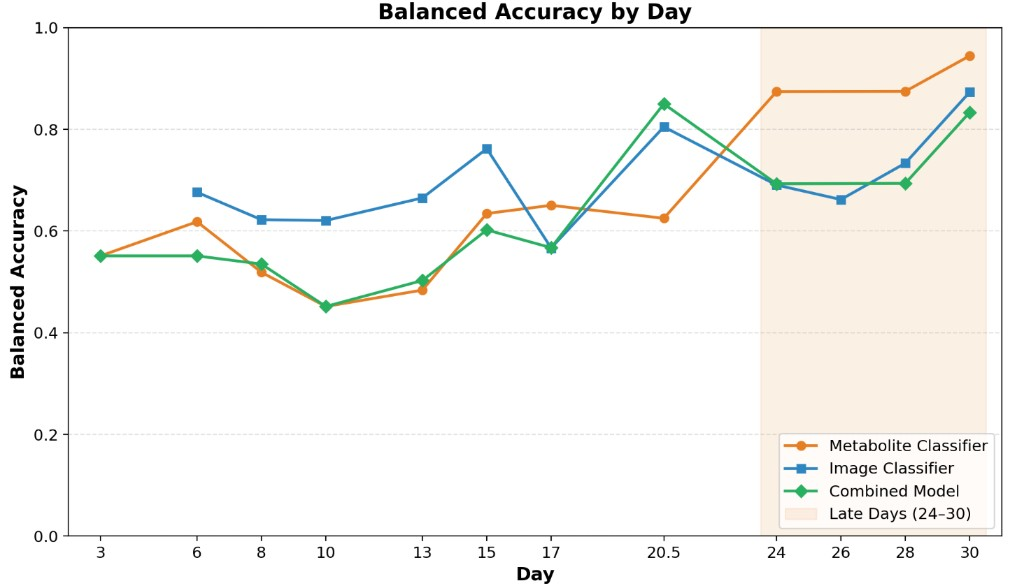
\includegraphics[width=0.85\textwidth]{Images/three_model.png}
  \caption{Comparison of the three models (image-only, metabolite-only, and combined) across days under the metric balanced accuracy.}
  \label{fig:three_models}
\end{figure}

\section{Results \& Comparison}

\subsection{Image Results}

Image-model results were reported under the overlay input setup (RGB with organoid outline), using the same train/ validation/ test split as the rest of the study. To allow direct comparison with the metabolite and combined models, all image results in this section used a fixed decision threshold of 0.5 on the predicted probability of the \textit{Acceptable} class. Balanced accuracy at this fixed threshold is the primary metric.

In the three-way comparison across models (Figure~\ref{fig:three_models}), the image classifier (per-day EfficientNet) performed strongly in the early and middle days, often leading the metabolite and combined models. It reached peaks of approximately 0.68 at Day 06 and 0.76 at Day 15, then dropped to about 0.57 at Day 17, an expected drop discussed below. After a recovery to roughly 0.81 at Day 20.5, balanced accuracy eased to about 0.68--0.69 at Day 24 and Day 26, then rose again to approximately 0.88 at Day 30. In the late-day window (Day 24--Day 30), the metabolite classifier achieved the highest balanced accuracy, while the image classifier remained competitive and the combined model fell below the two.

\subsubsection{Per-Day and Time-Series Comparison}

We compared two EfficientNet-based image models at the same fixed 0.5 threshold: a \textit{per-day} classifier (one model per day, using only the image at that day) and a \textit{time-series} model (one model per cutoff day, using the accumulated image sequence from Day 6 up to that day).

As shown in Figure~\ref{fig:perday_vs_timeseries}, the per-day model consistently outperformed the time-series model at every observed day. At Day 06 the per-day model reached balanced accuracy 0.68 versus 0.50 for the time-series model; at Day 15 the gap was 0.76 versus 0.48. The largest margin occurred at Day 20.5 (per-day 0.80, time-series 0.48). Even at Day 30, where both models improved, the per-day model reached 0.87 and the time-series model 0.67, a difference of 0.20 in balanced accuracy. The time-series model spent much of the early and middle period at or below random guessing chance (0.50): it fell to 0.48 at Day 10 and Day 13, and to its lowest point, 0.45, at Day 17. Only from Day 24 onward did it rise above 0.60, but it never matched the per-day model. In short, a single image at a given day outperformed the full accumulated growth history up to that date. This suggests that the current image carried more discriminative information than the temporal sequence, or that the time-series formulation was hampered by noise or representation issues from earlier days, where shapes of \textit{Acceptable} organoids and \textit{Not Acceptable} organoids did not diverge much. 

If the decision threshold was instead chosen per day by validation (e.g., to maximize balanced accuracy on the validation set), the time-series model could outperform the per-day model on the latest days (e.g., Day 28--Day 30). We did not treat that comparison as the primary result, because the validation-optimal threshold for the time-series model varied widely across days (from about 0.5 to 0.8), whereas the per-day model's optimal threshold remained stable around 0.5. That instability made it difficult to compare the two formulations on equal footing: the time-series gains at late days depended on day-specific thresholds that would be impractical to deploy without validation data at each time point, while the per-day model's consistent threshold supported a single, interpretable operating point.


Both image models showed a dip in balanced accuracy around Day~17 (Figure~\ref{fig:perday_vs_timeseries}). The per-day model fell from 0.76 at Day 15 to 0.57 at Day 17, and the time-series model reached its minimum of 0.45 at Day 17. The same dip is visible in the three-way comparison (Figure~\ref{fig:three_models}), where the image classifier drops to roughly 0.57 while the combined model also dips to about 0.56. 

This ``Day~17 drop'' pattern had a direct visual evidence (Figure~\ref{fig:day15_vs_day17}): in the image, the organoid at Day 17 was visibly smaller in size than at Day 15, a reduction that was obvious to the naked eye. That apparent shrinkage may confound the image models(e.g., by altering scale or boundary size in the overlay) and contributed to the dip in balanced accuracy. This inconsistency partially explained why image-based quality prediction was not uniformly strong across days, and the time-series model suffered particularly from the sudden shrinkage of images. 

\begin{figure}[htbp]
  \centering
  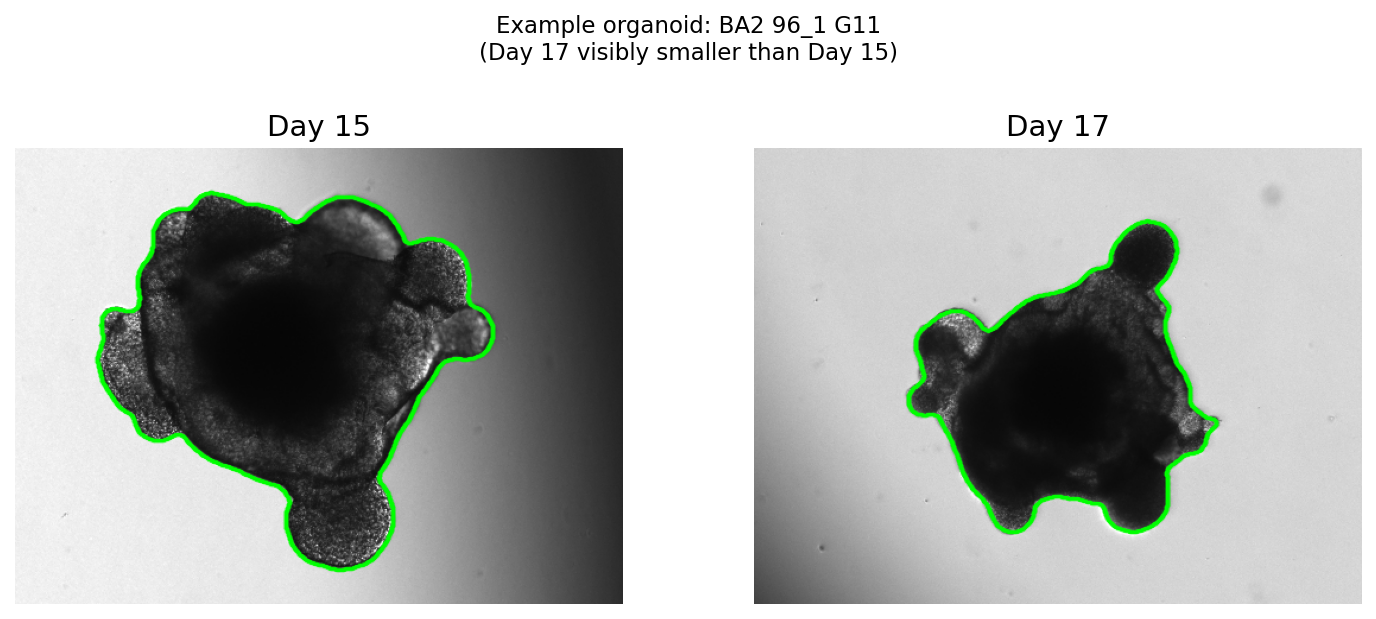
\includegraphics[width=0.85\textwidth]{Images/day15_vs_day17_overlays.png}
  \caption{Comparison of a specific organoid overlays image at Day~15 versus Day~17, illustrating the size change associated with the ``Day~17 drop'' pattern.}
  \label{fig:day15_vs_day17}
\end{figure}

\subsection{Metabolite Results}

\begin{figure}[H]
    \centering
    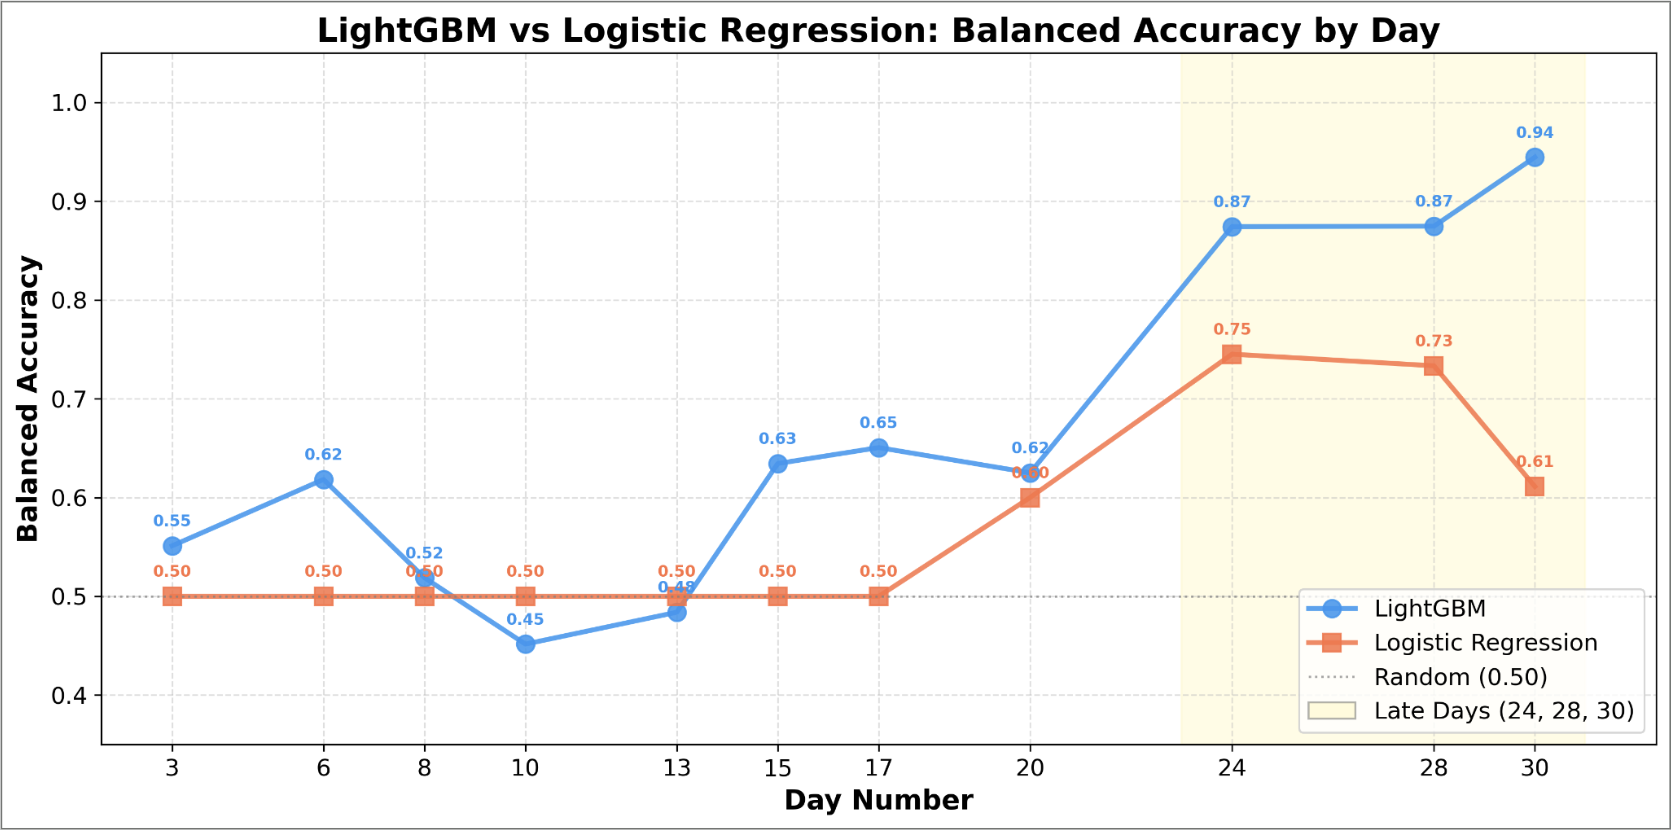
\includegraphics[width=0.9\textwidth]{Images/LightGBM_vs_Logistic_Regression.png}
    \caption{Balanced accuracy by day for LightGBM and logistic regression on metabolite-only prediction. LightGBM outperforms logistic regression at most time points and shows especially large gains at later days. The shaded region highlights the late-stage period (Days 24, 28, and 30).}
    \label{fig:lightgbm_vs_logreg}
\end{figure}

The logistic regression baseline produced deceptively strong overall accuracy in the early and middle days, but balanced accuracy exposed the underlying failure mode. From Day 03 through Day 17, test accuracy stayed near $0.84$, yet balanced accuracy remained fixed at $0.50$ because the model was almost entirely predicting the majority \textit{Acceptable} class. In confusion-matrix terms, it generated many true positives for \textit{Acceptable} organoids and very few false positives against them, but it did so by collapsing the minority class: \textit{Not Acceptable} organoids were almost always absorbed into the \textit{Acceptable} prediction group, producing persistent false negatives and zero recall for the \textit{Not Acceptable} class. This is why the \textit{Acceptable}-class metrics looked artificially strong in that period: recall for \textit{Acceptable} was $1.00$, while recall for \textit{Not Acceptable} was $0.00$. Precision followed the same imbalance in usefulness, since the model rarely made minority-class predictions at all. Starting at Day 24, logistic regression did begin to recover some minority-class signal. Balanced accuracy rose to roughly $0.75$ at Day 24 and $0.73$ at Day 28 as the model produced more true negatives and fewer missed poor-quality organoids. However, the drop at Day 30, where balanced accuracy fell to roughly $0.61$ and \textit{Not Acceptable} recall fell back to $0.22$, suggests that these late-day gains were not fully stable. In other words, logistic regression improved once the metabolite signal became stronger, but the final-day decline is a warning that its predictions were still not reliable enough to treat as the primary metabolite result.

LightGBM improved on that baseline by recovering minority-class signal much earlier, even when early-day performance remained limited in absolute terms. In the early and middle days, its overall accuracy was sometimes similar to or slightly below logistic regression, but the error structure was materially better. At Day 06, for example, LightGBM achieved the same overall accuracy as logistic regression ($0.81$) while increasing balanced accuracy to approximately $0.62$, because it no longer ignored the \textit{Not Acceptable} class entirely. Instead of producing only false negatives for poor-quality organoids, it began converting a subset of those cases into true negatives, raising \textit{Not Acceptable} recall to $0.33$ and \textit{Not Acceptable} precision to $0.40$. Similar gains persisted through Day 15 and Day 17. The main point is not that LightGBM solved the early-day problem, since it did not, but that it changed the kind of mistake being made: rather than defaulting almost completely to the majority class, it began detecting some minority-class cases without overwhelming the \textit{Acceptable} class with false alarms.

The strongest LightGBM results emerged at the late time points, beginning at Day 24. At Day 24 and Day 28, it reached overall accuracy of roughly $0.93$ and balanced accuracy of roughly $0.87$, clearly outperforming logistic regression on both summary measures. More importantly, the confusion matrix became well balanced across classes. For \textit{Acceptable} organoids, recall remained very high ($0.97$ at both Day 24 and Day 28), so the model was still preserving the majority class. For \textit{Not Acceptable} organoids, recall rose to $0.78$ at both days, meaning that most poor-quality organoids were now being caught rather than missed. Precision also improved sharply on the minority side, reaching $0.88$ at both Day 24 and Day 28, which means that when the model flagged a poor-quality organoid, it was usually correct. In practical terms, the remaining errors at these late days were relatively limited: a small number of false positives against \textit{Acceptable} organoids and a small number of false negatives on \textit{Not Acceptable} organoids, rather than the one-sided collapse seen in logistic regression.

Day 30 was the clearest demonstration of why we selected LightGBM as the final metabolite model. It achieved $0.98$ overall accuracy and approximately $0.94$ balanced accuracy, which was the strongest metabolite-only result in the study. The breakdown of errors is even more informative than the summary metrics. The model correctly identified every \textit{Acceptable} organoid in the test set, giving \textit{Acceptable}-class recall of $1.00$, and it achieved \textit{Acceptable}-class precision of $0.97$. For the \textit{Not Acceptable} class, precision was $1.00$, meaning every organoid flagged as poor-quality was truly poor-quality, while recall was $0.89$, indicating that only one poor-quality organoid was missed. In confusion-matrix terms, the model produced no false positives for the minority class and only a single false negative. That pattern is much closer to the practical screening objective of the project: preserve \textit{Acceptable} organoids while also identifying poor-quality ones with very little ambiguity.

These results also clarify why the final training choices mattered. The gain from LightGBM was not only that it produced better accuracy and balanced accuracy. It also shifted the error profile in the right direction for the application. A linear model that defaults toward the majority class can appear \textit{Acceptable} under raw accuracy, but it fails at the point where the screening task is most valuable: identifying poor-quality organoids before they are treated as \textit{Acceptable}. The final LightGBM configuration addressed that problem in three coordinated ways. First, the tree-based architecture could represent nonlinear relationships and interactions among metabolite features. Second, class weighting prevented the minority class from being washed out during fitting. Third, threshold tuning against the \textit{Not Acceptable} F1 score pushed selection toward a better balance between false positives and false negatives on the class that mattered most.

Overall, the metabolite results support two direct conclusions. First, metabolite differences alone carried limited class-separating signal in the earliest days, so weak early minority-class performance should not be treated as purely an algorithmic failure. Second, once the organoids reached later stages, those same features became much more informative, and LightGBM converted that late-day signal into strong performance both overall and across classes. For that reason, logistic regression is best understood as a useful baseline, while LightGBM with concentration differences is the primary metabolite model reported in the paper.

\subsubsection{Feature Importance}

To better understand how metabolite signals contributed to classification across the developmental timeline, we examined feature importance values from the LightGBM metabolite classifier. The analysis included both absolute metabolite concentrations and day-to-day differences in those concentrations for each organoid. Figure~\ref{fig:feature_importance} summarizes the relative importance of these features at four representative time points: Days 6, 15, 24, and 30. Because each day-specific model was trained independently, the feature rankings reflect stage-specific predictive signals rather than a single unified model.

At Day 6, the classifier relied primarily on absolute concentration features, particularly glutamate and lactate. By Day 15, the difference in lactate concentration became the single most important feature, suggesting that short-interval changes in lactate carry predictive signals during mid-development. At Day 24, the model showed a more balanced mixture, with both concentration and difference features contributing. Glucose and pyruvate features followed a general downward trend across the timeline and became less influential in later models.
Malate exhibited the most distinctive temporal pattern. Because malate measurements were only available after Day 10, malate features were absent from the earliest models. By Day 30, however, the difference in malate concentration emerged as the most important feature overall. This late-stage prominence is consistent with metabolic divergence between organoids becoming more pronounced as maturation proceeds.

Across the timeline, feature importance shifted gradually from concentration-dominant predictors in early development toward greater influence from difference features at later stages. These difference features capture directional changes in metabolite levels between consecutive observations, allowing the model to distinguish organoids with similar absolute concentrations but different metabolic trajectories. Taken together, these patterns reinforce the broader metabolite results: early-stage signals provided limited class separation, while lactate and malate became increasingly informative at later time points, consistent with the stronger classification performance observed at Days 24 and 30.

\begin{figure}[H]
\centering
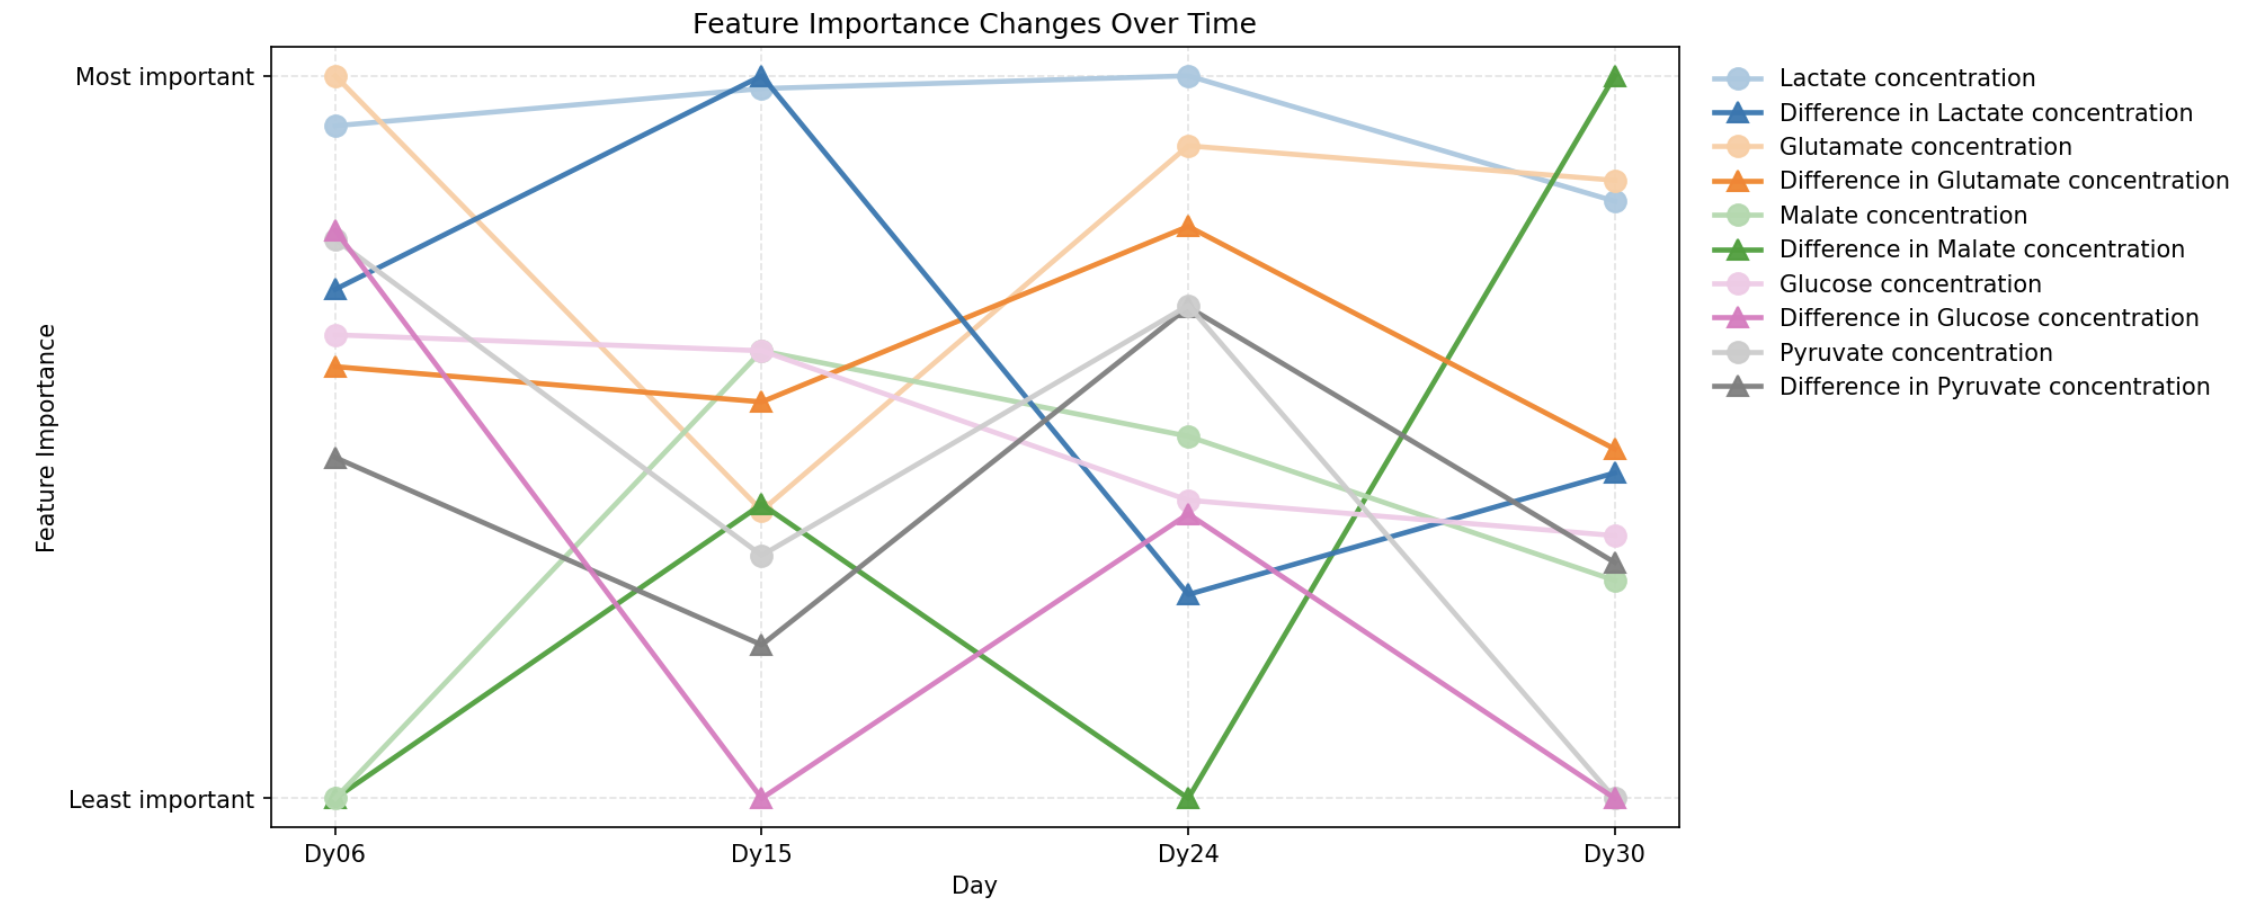
\includegraphics[width=0.85\textwidth]{Images/Feature Importance Graph.png}
\caption{Feature importance from the LightGBM metabolite classifier across selected days. Circle markers denote absolute metabolite concentrations, while triangle markers denote differences in concentration between consecutive observations.}
\label{fig:feature_importance}
\end{figure}

\subsection{Combined Model Results}

Across reproducibility runs with multiple seeds, the combined model showed a consistent temporal pattern: performance was modest at early and mid time points and improved at late time points (Day 24--Day 30). Quantitatively, balanced accuracy was limited through approximately Day 17 (mean balanced accuracy $\approx 0.57$ across seeds), but increased at late days (Day 24--Day 30: mean balanced accuracy $\approx 0.76$ across seeds).

The balanced-accuracy curves suggested that, in early days, the combined model often tracked the metabolite-only classifier more closely than the image-only classifier, consistent with the idea that early morphology was not yet strongly differentiated, while chemical measurements may have captured subtle differences in metabolic state. In contrast, by late days, the organoids' shapes diverged more clearly, and images contributed more visibly; both models proved to carry more signals at later time points, as mentioned earlier. 

However, the combined model did not eliminate the core early-day limitation: when ground-truth labels were derived from late-day assessments and propagated backward, early-day predictors may have legitimately lacked a separable signal, and the small number of \textit{Not Acceptable} examples per day made specificity-based metrics fragile. 

Overall, the combined model was most compelling as a screening tool at late time points, when both image and metabolite data of two classes of organoids had diverged. Future improvements were likely to come from (i) collecting more confidently labeled \textit{Not Acceptable} organoids, (ii) learning combined strategies that adapt by day (rather than a fixed PCA+concatenation scheme), and (iii) extending experiments to a time-series backbone, where cumulative evidence of the combination of two types of data may be more informative.

\section{Conclusion}

\subsection{Findings}

First, image-based data provided useful predictive signal across almost all of the growth period, with balanced accuracy higher than 0.6 in almost all measurement days. The per-day EfficientNet classifier reached relatively high balanced accuracy at early and middle days (e.g., 0.76 at Day~15) and again at Day~30 (0.88), with only a pronounced dip at Day 17 that coincided with a visible size reduction in the images. 

Second, a single image at a given day outperformed a time-series model that used the accumulated image sequence from Day~6 onward, suggesting that the current image carried more discriminative information than the temporal sequence before that time point, if an image classifier were to be deployed. 

Third, metabolite-only prediction was weaker in early days but became stronger at late time points than the image-only prediction. LightGBM with concentration and difference features achieved the best metabolite result at Day~30 (balanced accuracy $\approx$ 0.94) and recovered minority-class signal much earlier than a logistic regression baseline. A late period prediction would be more accurate when deploying a metabolite-only classifier. 

Fourth, the combined model did not consistently outperform the better of the two models at any given day. It tracked the metabolite model more closely in early days and improved at late days, but the practical gain over a single-model deployment was limited under the current fusion design, though having a great potential to benefit from the better of the two models at any specifically given time point.

These results have direct implications for organoid screening. Metabolite-based models are most informative in late days and can be used alone or in combination with images when early-day prediction must be made. The relative strength of image versus metabolite signal depends on the day, so deployment choices can be day-specific rather than one-size-fits-all, although the metabolite model was overall the best choice. 

\subsection{Limitations and Future Improvements}

There were also some limitations we failed to resolve throughout the project. Firstly, the backward propagation of late-stage labels to earlier time points may leave early-day predictors with limited separable signal, especially in the early stage of growth all organoid images looked relatively similar. Secondly, the limited number of \textit{Not Acceptable} examples per day created extreme minority on this class versus the \textit{Acceptable} class, leaving the models less predictive power over the \textit{Not Acceptable} class. Thirdly, the fixed PCA-plus-concatenation fusion in the combined model may not fully exploit interactions between the two models, as currently it did not consistently beat the better of the two models. 

Future work could explore day-adaptive combination techniques, time-series formulations that incorporate both image and metabolite history, and collection of more confidently labeled \textit{Not Acceptable} class organoids to stabilize minority-class evaluation.


\bibliographystyle{plainnat}
\bibliography{references}

\end{document}